\section{Overview}
\label{sec:overview}

\begin{figure}
	\centering
	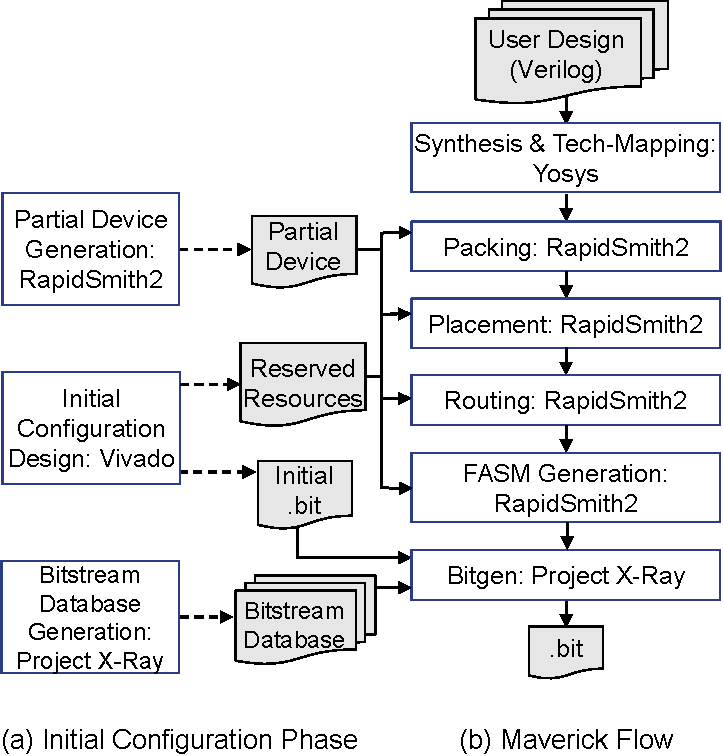
\includegraphics[height=.83\columnwidth]{figures/flow_overview.pdf}
	\caption{(a) The Initial Configuration Phase. (b) The Stand-alone Maverick 
		Design Flow.}
	\label{fig:overview}
\end{figure}

Like the tool flows just mentioned, the Maverick design flow is a CAD flow that can generate configuration bitstreams for commercial FPGAs.
The Maverick flow is designed to target a PR region of an FPGA rather than a full FPGA device. 
This PR region acts as a miniature FPGA for the circuits created with the Maverick flow. 
The bitstreams generated by the Maverick flow are thus {\em partial} bitstreams that configure a PR region of the FPGA within a static, pre-configured {\em initial} base design.

Before the Maverick flow can be used, a static system must first be created on a computer that can run Vivado.
The creation of this static system results in a set of files that describe the static base design and the PR region in which user designs can be implemented.
Once this static system has been created, the Maverick flow can be run to compile user designs to partial bitstreams.

The Maverick flow first uses Yosys to synthesize and tech-map designs.
In contrast to previous tool flows, Maverick then uses RapidSmith2-based tools to pack, place, and route the design.
To perform these steps, a partial device model created with the Vivado Design Interface (VDI) and RapidSmith2 must be used.
Finally, Maverick uses the Project X-Ray tools for bitstream generation.

The Maverick flow can be targeted to any platform that can support each of these tools. 
The minimum requirements for running the Maverick flow include a Java runtime environment (JRE), a Python interpreter, a {\tt C++} compiler, sufficient memory (dependent upon PR region and design size), and at least 30 MB of disk space for the tools.
This allows the Maverick flow to run on smaller embedded platforms, such as an ARM processor on a Xilinx Zynq SoC.
